\chapter{Automated artifact rejection for M/EEG}
\label{chapter:autoreject}

\epigraph{\small\itshape ``With four parameters I can fit an elephant, and with five I can make him wiggle his trunk.''}{\small\textit{---John von Neumann}}

\begin{figure}[ht!]
\centering
\begingroup
\etocstandardlines
%\renewcommand{\etocbkgcolorcmd}{\color{lightgray}}
\renewcommand{\etocbelowtocskip}{0pt\relax}
\fboxsep1ex
\etocframedstyle [1]{\fbox{\makebox[.4\linewidth]{\etocfontminusone
Contents}}}
\localtableofcontents
\endgroup
\end{figure}

\clearpage

In the last chapter, we discussed the reproducibility challenges when performing group studies in \ac{MEG} and \ac{EEG}. One of the ways to improve reproducibility is automation, and we briefly touched upon an algorithm for automating detection of bad data segments, known as \emph{autoreject}.

%copy pasted abstract below
In this chapter, we will present this algorithm which rejects and repairs bad trials in \ac{MEG} and \ac{EEG} signals. The method capitalizes on cross-validation in conjunction with a robust evaluation metric to estimate the optimal peak-to-peak threshold - a quantity commonly used for identifying bad trials in M/EEG. This approach is then extended to a more sophisticated algorithm which estimates this threshold for each sensor yielding trial-wise bad sensors. Depending on the number of bad sensors, the trial is then repaired by interpolation or by excluding it from subsequent analysis. All steps of the algorithm are fully automated thus lending itself to the name \emph{autoreject}. In order to assess the practical significance of the algorithm, we conducted extensive validation and comparisons with state-of-the-art methods on four public datasets containing \ac{MEG} and \ac{EEG} recordings from more than 200 subjects. The comparisons include purely qualitative efforts as well as quantitatively benchmarking against human supervised and semi-automated preprocessing pipelines. The algorithm allowed us to automate the preprocessing of \ac{MEG} data from the \ac{HCP} going up to the computation of the evoked responses. The automated nature of our method minimizes the burden of human inspection, hence supporting scalability and reliability demanded by data analysis in modern neuroscience.

\noindent\fcolorbox{white}{lightgray}{%
\begin{minipage}{\dimexpr\textwidth-2\fboxrule-2\fboxsep\relax}
\begin{itemize}[align=left, leftmargin=10pt, labelwidth=5pt, labelindent=10pt, itemsep=5pt, topsep=5pt]
  \item[] Section~\ref{sec:introduction} to Section~\ref{sec:autoreject_conclusion} was published in:
  \item \bibentry{jas2016automated}
  \item \bibentry{jas2017autoreject}
\end{itemize}
\end{minipage}}%

\clearpage
\section{Introduction}
\label{sec:introduction}

\begin{figure}[t]
	\centering
	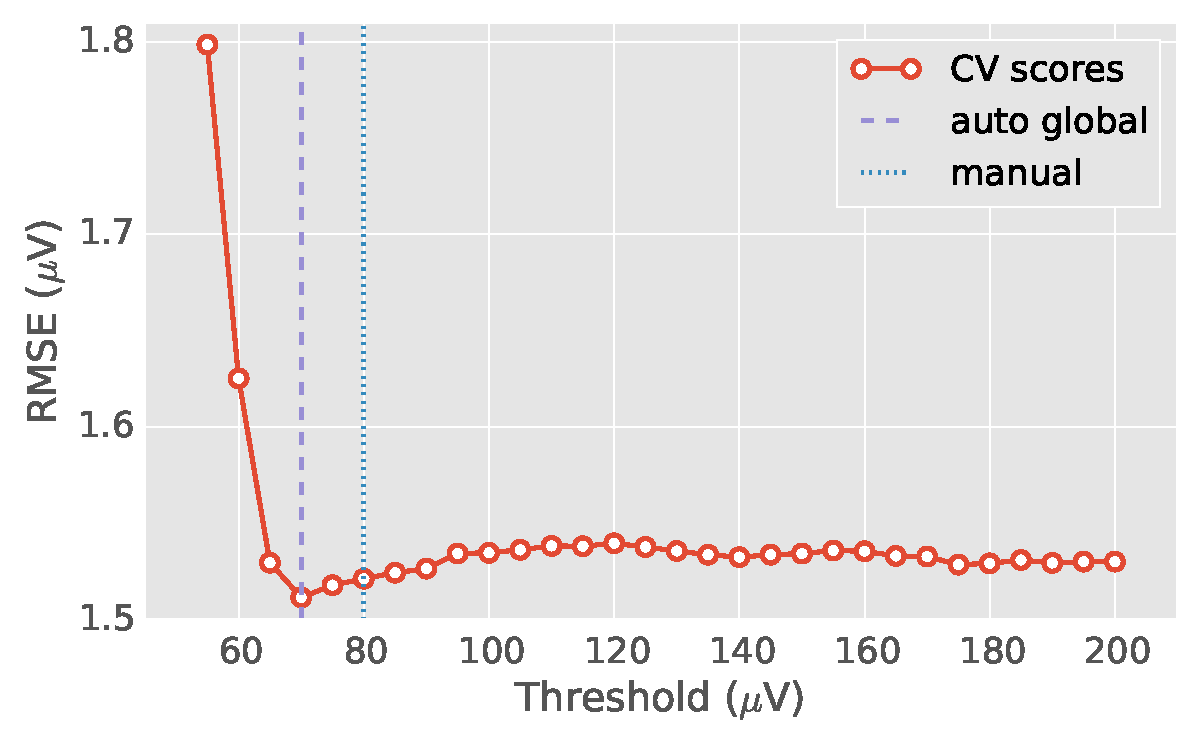
\includegraphics[width=0.65\linewidth]{figures/figure1.pdf}
    \caption[Cross-validation error as a function of peak-to-peak rejection threshold on one EEG dataset.]{Cross-validation error as a function of peak-to-peak rejection threshold on one EEG dataset. The root mean squared error (RMSE) between the mean of the training set (after removing the trials marked as bad) and the median of the validation set was used as the cross-validation metric (Section~\ref{sec:auto_global}). The two insets show the average of the trials as ``butterfly plots" (each curve representing one sensor) for very low and high thresholds. For low thresholds, the RMSE is high because most of the trials are rejected (underfit). At high thresholds, the model does not drop any trials (overfit). The optimal data-driven threshold (\emph{autoreject, global}) with minimum RMSE is somewhere in between. It closely matches the human threshold.}
    \label{fig:cross_val}
\end{figure}

Magneto-/electroencephalography (M/EEG) offer the unique ability to explore
and study, non-invasively, the temporal dynamics of the brain and its cognitive processes. The M/EEG community has only recently begun to appreciate the importance of large-scale studies, in an effort to improve replicability and statistical power of experiments. This has given rise to the practice of sharing and publishing data in open archives~\citep{gorgolewski2016practical}. Examples of such large electrophysiological datasets include the Human Connectome Project (HCP)~\citep{van2012human, larson2013adding}, the Physiobank~\citep{goldberger2000physiobank}, the OMEGA archive~\citep{niso2016omega} and Cam-CAN~\citep{taylor2015cambridge}. A tendency towards ever-growing massive datasets as well as a shift towards common standards for accessing these databases~\citep{gorgolewski2016brain,bigdely2013hierarchical} is clearly visible. The UK Biobank project~\citep{ollier2005uk} which currently hosts data from more than 50,000 subjects is yet another example of this trend.

This has however, given rise to new challenges including automating the analysis pipeline~\citep{gorgolewski2016practical}. Automation will not only save time, but also allow scalable analysis and reduce the barriers to reanalysis of data, thus facilitating reproducibility. \citet{engemann2015automated_new} have recently worked towards more automation in M/EEG analysis pipelines by considering the problem of covariance estimation, a step commonly done prior to source localization. Yet, one of the most critical bottlenecks that limits the reanalysis of M/EEG data remains at the preprocessing stage with the annotation and rejection of artifacts. Despite being so fundamental to M/EEG analysis given how easily such data can be corrupted by noise and artifacts, there is currently no consensus in the community on how to address this particular issue.

In the presence of what we will refer to as \emph{bad} data, various data cleaning strategies have been employed. A first intuitive strategy is to exclude bad data from analysis, to \emph{reject} it. While this approach is very often employed, for example, because data cleaning is time consuming, or out
of reach for practitioners, it leads to a loss of data that are costly to acquire. This is particularly the case for clinical studies, where patients have difficulties staying still or focusing on the task~\citep{cruse2012bedside,goldfine2013reanalysis}, or even when babies are involved as subjects~\citep{basirat2014hierarchy}.

When working with M/EEG, the data can be bad due to the presence of bad sensors (also known as channels\footnote{They are not necessarily equivalent in the case of a bipolar montage in EEG. However, for the sake of simplicity, we shall use these terms interchangeably in this work.}) and bad trials.
A trial refers here to a data segment whose location in time is typically related to an experimental protocol. But here we will also call trial any data segment even if it is acquired during a task-free protocol.
Accordingly, a bad trial or bad sensor is one which contains bad data.
%
Ignoring the presence of bad data can adversely affect analysis downstream in the pipeline. For example, when multiple trials time-locked to the stimulation are averaged to estimate an evoked response,
ignoring the presence of a single bad trial can corrupt the average. The mean of a random vector is not robust to the presence of strong outliers. Another example quite common in practice, both in the case of EEG and MEG, is the presence of a bad sensor. When kept in the analysis, an artifact present on a single bad sensor can spread to other sensors, for example due to spatial projection. This is why identifying bad sensors is crucial for data cleaning techniques such as the very popular Signal Space Separation (SSS) method~\citep{taulu2004suppression}. Frequency filtering~\citep{widmann2015digital} can often suppress many low frequency artifacts, but turns out to be insufficient for broadband artifacts. A common practice to mitigate this issue is to visually inspect the data using an interactive viewer and mark manually, the bad sensors and bad segments in the data. Although trained experts are very likely to agree on the annotation of bad data, their judgement is subject to fluctuations and cannot be repeated. Their judgement can also be biased due to prior training with different experimental setups or equipments, not to mention the difficulty for such experts to allocate some time to review the raw data collected everyday.
% \fede{Experts do not only self-bias from the first inspection to the last one (been there), but also are biased by the kind of analysis. For example: sleep/awake data. I could easily mark as bad trials when there are micro-awakes during sleep, helping a multivariate classifier separate those conditions. The difficult thing is doing blind and unbiased cleaning. If we could set up a clear set of rules on when to reject data, then we have an algorithm, and then we can program it. So by definition, there is no such thing as an algorithm that drives the experts into data cleaning without bias. Even though the main reason for an automatic method to exist is because of big databases, the cleaning/rejecting problem is present even with a few recordings.}

Luckily, popular software tools such as
Brainstorm~\citep{tadel2011brainstorm}, 
EEGLAB~\citep{delorme2004eeglab}, 
FieldTrip~\citep{oostenveld2010fieldtrip},
MNE~\citep{gramfort2013meg}
or SPM~\citep{litvak2011eeg} already allow for the rejection of bad data segments based on simple metrics such as peak-to-peak signal amplitude differences that are compared to a manually set threshold value. When the peak-to-peak amplitude in the data exceeds a certain threshold, it is considered as bad. However, while this seems quite easy to understand and simple to use from a practitioner's standpoint, this is not always convenient. In fact, a good peak-to-peak signal amplitude threshold turns out to be data specific, which means that setting it requires some amount of trial and error.
% \fede{The problem of cleaning by peak-to-peak amplitude, at least in EEG, is that different systems, setups, subjects, locations, with the same stimulation and analysis, leads to different results. Our auditory paradigm that we’ve been recording since 2008 is a proof of that. They already changed the stimulation computer 2 times, but always using eprime. The EEG amplifier, although it’s the same brand, model, has indeed a different serial number, so different problems (we have one with channel 54 broken, and another with channel 14). Now we are using another stimulation device because the computer started to inject 15 Hz noise. So now we use pneumatic headphones, because we also had noise from the electronics in the bed the patients were. Depending on the department in the hospital in which the patient is, different problems may arise. Last one had a pacemaker and really broke everything.
% To summarise, my point is that it is not only data specific at a group level, but at a single recording level. And doing group analysis and statistics when rejecting rules are not clear can lead to biased results and even false positives.}

The need for better automated methods for data preprocessing is clearly shared by various research teams, as the literature of the last few years can confirm. On the one hand, are pipeline-based approaches, such as Fully Automated Statistical Thresholding for EEG artifact rejection (FASTER by~\citet{nolan2010faster}) which detect bad sensors as well as bad trials using fixed thresholds motivated from classical Gaussian statistics. Methods such as PREP~\citep{bigdely2015prep}, on the other hand, aim to detect and clean the bad sensors only. Unfortunately, they do not offer any solution to reject bad trials. Other methods are available to solve this problem. For example, the Riemannian Potato~\citep{barachant2013riemannian} technique can identify the bad trials as those where the covariance matrix lies outside of the ``potato'' of covariance matrices for good trials. By doing so, it marks trials as bad but does not identify the sensors causing the problem, hence not offering the ability to repair them. It appears that practitioners are left to choose between different methods to reject trials or repair sensors, whereas they are in fact intricately related problems and must be dealt with together. 

Robust regression~\citep{diedrichsen2005detecting} also deals with bad trials using a weighted average which mitigates the effect of outlier trials. Trials with artifacts end up with low contributions in the average. A related approach that is sometimes employed to ignore outlier trials in the average is the trimmed mean as opposed to a regular mean. The trimmed mean is a compromise between the mean which offers a high signal-to-noise ratio (SNR) but can be corrupted by outliers, and the median which is immune to outliers of extreme amplitudes but has a low SNR as it involves no averaging. Of course, neither of these strategies are useful when analyses have to be conducted on single trials. Another approach, which is also data-driven, is Sensor Noise Suppression (SNS)~\citep{de2008sensor}. It removes the sensor-level noise by spatially projecting the data of each sensor onto the subspace spanned by the principal components of all the other sensors. This projection is repeated in leave-one-sensor-out iterations so as to eventually clean all the sensors. In most of these methods, however, there are parameters which are somewhat dataset dependent and must therefore be manually tuned.

We therefore face the same problem in automated methods as in the case of semi-automated methods such as peak-to-peak rejection thresholds, namely the tuning of model parameters. In fact, setting the model parameters is even more challenging in some of the methods when they do not directly translate into human-interpretable physical units.
% \fede{Current automatic methods not only need manually tuned parameters, but in order to tune those parameters, deep knowledge of the underlying process. There's nothing with no paremeters like autoreject}

This led us to adopt a pragmatic approach in terms of algorithm design, as it focuses on the tuning of the parameters that M/EEG users presently choose manually. The goal is, not only to obtain high quality data but also to develop a method which is transparent and not too disruptive for the majority of M/EEG users. A first question we address below is: can we improve peak-to-peak based rejection methods by automating the process of trial and error? In the following section, we explain how the widely-known statistical method of cross-validation (see Figure~\ref{fig:cross_val} for a preview) in combination with Bayesian optimization~\citep{snoek2012practical, bergstra2011algorithms} can be employed to tackle the problem at hand. We then explain how this strategy can be extended to set thresholds separately for each sensor and mark trials as bad when a large majority of the sensors have high-amplitude artifacts. This process closely mimics how a human expert would mark a trial as bad during visual inspection. 

In the rest of the paper, we detail the internals of our algorithm, compare it against various state-of-the-art methods, and position it conceptually with respect to these different approaches. For this purpose, we make use of qualitative visualization techniques as well as quantitative reports. In a major validation effort, we take advantage of cleaned up evoked response fields (ERFs) provided by the Human Connectome Project~\citep{larson2013adding} enabling ground truth comparison between alternative methods. This work represents one of the first efforts in reanalysis of the MEG data from the HCP dataset using a toolkit stack significantly different from the one employed by the HCP consortium. The convergence between our method and the HCP MEG pipelines is encouraging and testifies to the success of the community-wide open science efforts aiming at reproducible research. Naturally, we have therefore made our code available online\footnote{\url{https://autoreject.github.io}}. In addition to this, we validated our algorithm on the MNE sample data~\citep{gramfort2013meg}, the multimodal faces dataset~\citep{wakeman2015multi}, and the EEGBCI motor imagery data~\citep{goldberger2000physiobank,schalk2004bci2000}.

A preliminary version of this work was presented in~\citet{jas2016automated}.
\paragraph{Notations} We denote matrices by capital letters $X \in \real^{m \times n}$. The $i$th row of a matrix is indexed by subscripts, as in $X_{i}$, and the entry in the $i$th row and $j$th column is indexed as $X_{ij}$. The matrix $X$ restricted to the rows with indices in the set $\mathcal{G}$ is denoted by $X_\mathcal{G}$. All sets $\mathcal{G}$, $\mathcal{T}$ or $\mathcal{V}$ are written in calligraphic fonts.
